Abbiamo previsto tre layout differenti basati sulla dimensione dello schermo del device client. Di seguito la pagina articoli vista da tre dispositivi diversi:
\begin{itemize}
	\item \bfseries{Desktop}:
		\begin{figure}[h]
		\centering
		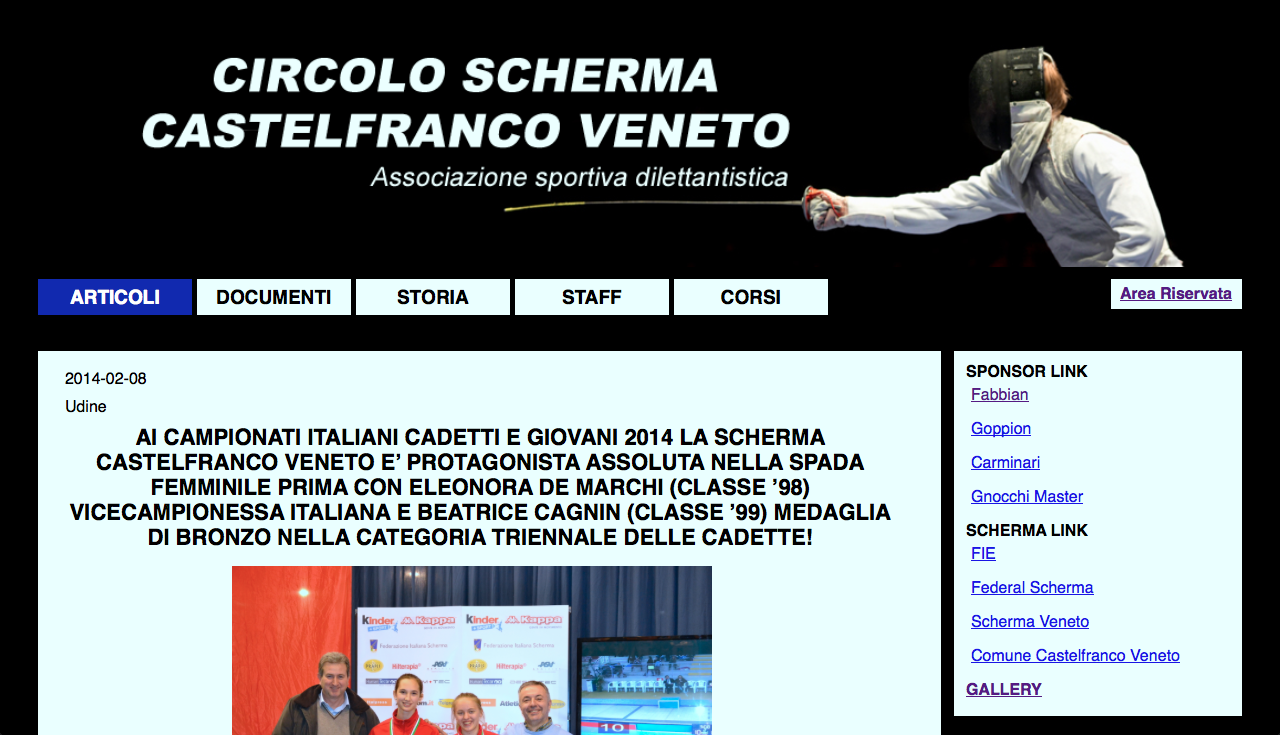
\includegraphics[scale=0.32]{images/articoli_desktop.png}
		\caption{Screenshot desktop articoli.cgi}
	\end{figure}
	\item \bfseries{Tablet}:
		\begin{figure}[h]
			\centering
			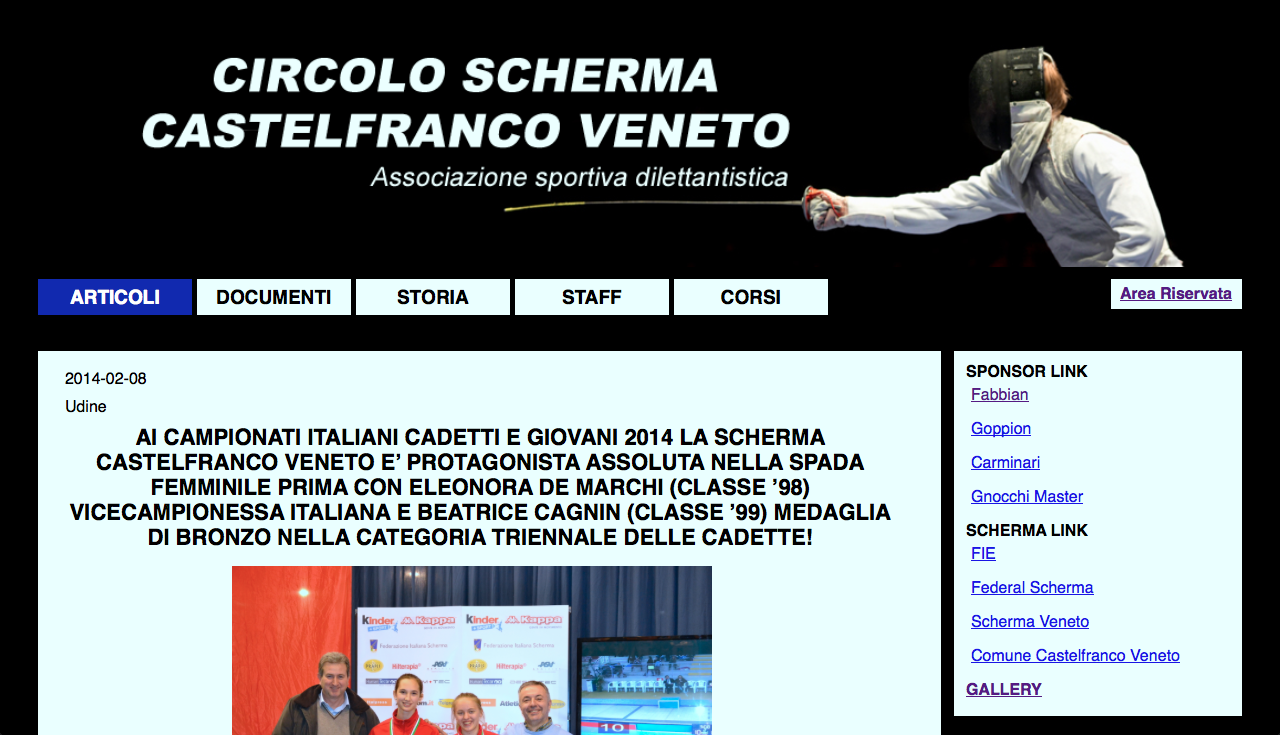
\includegraphics[scale=0.30]{images/articoli_tablet.png}
			\caption{Screenshot tablet articoli.cgi}
		\end{figure}
	\item \bfseries{Mobile}:
		\begin{figure}[h]
			\centering
			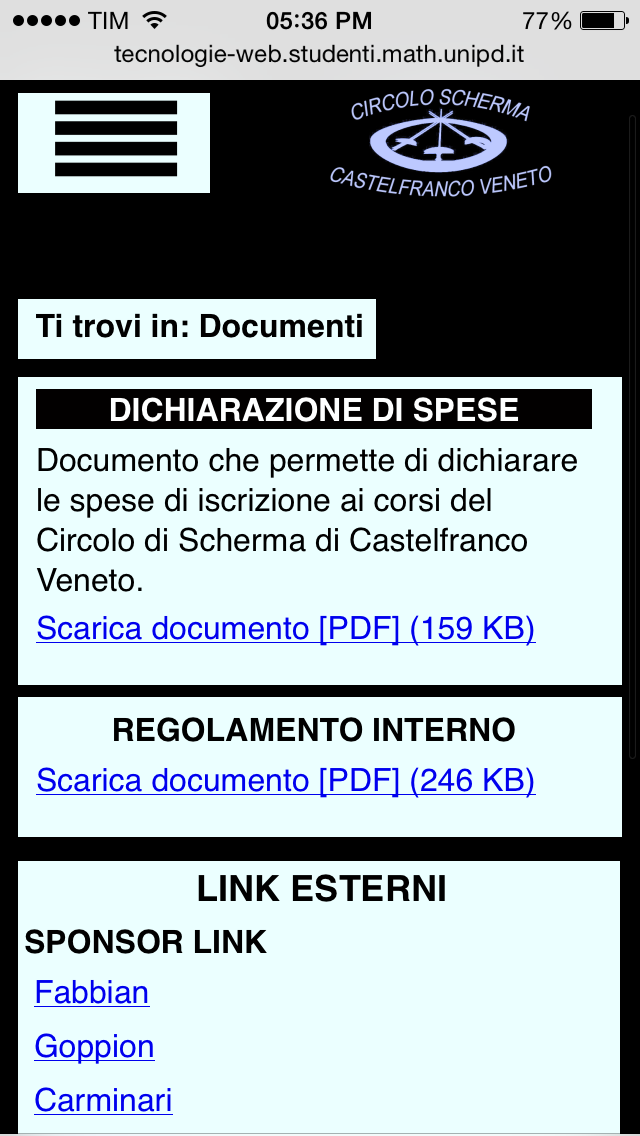
\includegraphics[scale=0.30]{images/articoli_mobile.png}
			\caption{Screenshot mobile articoli.cgi}
		\end{figure}
	
\end{itemize}
Sono previste delle variazione del layout nel caso javascript sia disabilitato nel browser client. In particolare nelle pagine di inserimento o modifica della parte amministratore, vengono nascosti i bottoni dei tag speciali e la sidebar con la legenda, per far spazio ad una colonna con le istruzioni per inserire i tag correttamente.